% --------------------------------------------------------------------------- %
% --------------------------------------------------------------------------- %
\chapter{The \texorpdfstring{\mttwo} VVariable Search}
\label{ch:analysis}

\section{Analysis Strategy}
\label{sec:strategy}
Searches for new physics targeting all-hadronic final states present unique challenges and opportunities at the LHC, and have previously been conducted by both the ATLAS collaboration \cite{Aad:2016jxj,Aaboud:2016tnv,Aaboud:2016zdn,Aad:2016eki,Aaboud:2016nwl,Khachatryan:2016epu} and the CMS collaboration \cite{Khachatryan:2016xvy,Khachatryan:2016kdk,Khachatryan:2016dvc}. While such searches typically implement stringent vetoes on lepton candidates and thus suppress the need to correctly identify ``real'' leptons, the high rate of QCD processes in proton-proton collisions generates large amounts of SM events with all-hadronic final states. Designing a search targeting signatures with all-hadronic final states requires a mechanism to distinguish and suppress the selection of multi-jet QCD events from new physics signatures, as well as robust background estimation methods to predict the yield of SM events which may generate true missing energy (such as \znunu).

The \mttwo analysis harnesses the discriminating power of the \mttwo variable, sometimes referred as stransverse mass, to distinguish SM events from possible signatures of new physics. By first requiring a significant amount of missing energy in the event, multi-jet QCD processes are greatly suppressed. Additional requirements on the topology of the event implemented using \mttwo further suppress QCD-like processes and favor events with real missing energy anti-aligned with the hadronic energy deposits in the detector. After estimating the minimal QCD contribution remaining by extrapolating from a region orthogonal to the signal selection, the only remaining backgrounds are leptonic events where the lepton failed reconstruction or identification (or ``lost-lepton'' events), and SM events creating real \MET in the form of neutrinos from a decaying Z boson recoiling against jets (or ``invisible Z'' events).

\section{The \texorpdfstring{\mttwo} VVariable}
\label{sec:mt2}
\mttwo is a particularly useful kinematic mass variable for final states where two particles decay (possibly in a chain) to a final state containing an invisible particle X of mass $m_X$ \cite{Lester:1999tx}. The typical transverse mass $M_T$ is defined in equation \ref{eq:mt} for particles $i=1,2$, where the mass $m^{\text{vis}(i)}$, transverse momentum $\vec{p}_t^{\text{vis}(i)}$, and transverse energy $E_T^{\text{vis}(i)}$ characterize the visible kinematics of the decay chain, and $\vec{p}_t^{\text{X}(i)}$ and $E_T^{\text{X}(i)}$ characterize the unknown kinematics of the invisible particle X.
\begin{equation}
	(M_T^{(i)})^2 = (m^{\text{vis}(i)})^2 + m_{\text{X}}^2+2\left(E_T^{\text{vis}(i)} \cdot E_T^{\text{X}(i)} - \vec{p}_t^{\text{vis}(i)} \cdot \vec{p}_t^{\text{X}(i)} \right)
	\label{eq:mt}
\end{equation}
In principle, if the correct values of $m_{\text{X}}$ and $\vec{p}_t^{\text{X}(i)}$ were accessible, then the transverse mass would have a kinematic endpoint and not exceed the mass of the parent particles (disregarding any resolution effects). However, the individual momenta of the invisible particles in the two decay chains cannot be measured; the only quantity experimentally accessible is the total missing momentum $\vec{p}_T^{\text{miss}}$. With this in mind, the generalized transverse mass variable \mttwo is defined in equation \ref{eq:mt2}, where the unknown mass $m_{\text{X}}$ is a free parameter and a minimization is performed over the sum of invisible momenta $\vec{p}_t^{\text{X}(i)}$ that satisfy the measured $\vec{p}_T^{\text{miss}}$ constraint.
\begin{equation}
	M_{\text{T2}}(m_{\text{X}}) = \min_{\vec{p}_t^{\text{X}(1)}+\vec{p}_t^{\text{X}(2)}=\vec{p}_T^{\text{miss}}} \left[\max \left( M_T^{(1)},M_T^{(2)} \right) \right]
	\label{eq:mt2}
\end{equation}

Because this analysis selects final states with multiple jets in the final state, the calculation of \mttwo first requires grouping the hadronic jet activity into two large {\it pseudojets} to act as the visible components in the \mttwo equation. The jet activity in each event is divided into two hemispheres, and the jets in each hemisphere are summed together to created the pseudojets. The hemisphere algorithm proceeds as follows:
\begin{itemize}
	\item The direction of the two jets with largest invariant mass is chosen as the initial seed for the two axes.
	\item Jets are associated to one of the two axes according to the minimal Lund distance \cite{Ball:2007zza}, such that jet $k$ is associated to hemisphere $i$ instead of $j$ if the condition in equation \ref{eq:lundDist} is true.
	\item After each jet is associated to one of the two axes, the axes are recalculated by summing the momenta of all jets associated to an axis.
	\item The association algorithm iterates using the new axes, and continues until no jets are associated to a different axis after an iteration.
\end{itemize}
\begin{equation}
	(E_i - p_i \cos \theta_{ik}) \frac{E_i}{(E_i+E_k)^2} \leq (E_j - p_j \cos \theta_{jk}) \frac{E_j}{(E_j+E_k)^2} 
	\label{eq:lundDist}
\end{equation}
When clustered using this pseudojet algorithm, QCD multijet events may yield high \mttwo if the pseudojets have high jet masses, thus the visible masses $m^{\text{vis}(i)}$ are set to zero to suppress such SM events. Since the kinetic components of \mttwo will be large for signal events, this suppression does not isgnificantly impact sensitivity to many BSM signatures, thus \mttwo is calculated in this analysis using only \MET and the two pseudojets with $m_{\text{X}}\equiv 0$.


\section{Event Selection Criteria}
\label{sec:eventSelection}
The general strategy for the event selection is to first apply baseline cuts motivated by hardware and software-level triggers (discussed in section \ref{subsec:triggers}) and reducing the QCD multi-jet background to negligible levels. Events are further categorized using stransverse mass (\mttwo), the scalar sum of the transverse momenta \pt of all selected jets (\HT), the total number of jets in the event (\nj), and the total number of b-tagged jets in the event (\nb). A summary of the event preselections can be found in table \ref{tbl:selections}.
\begin{table}
	\centering
	\renewcommand{\baselinestretch}{1.0}
	\caption[Summary of physics objects and preselection for signal events.]{Summary of physics objects and preselection for signal events. Here $R$ is the distance parameter of the anti-\kt algorithm, and for veto leptons and tracks, the transverse mass \Mt is determined using the veto object and the $\vec{\MET}$, while $\pt^{\mathrm{sum}}$ denotes the sum of the transverse momenta of all the PF candidates in a cone around the lepton or track. The size of the cone, in units of $\Delta R \equiv \sqrt{\left(\Delta \phi\right)^2 + \left(\Delta \eta\right)^2}$ is given in the table. }
	 \begin{tabular}{ l | l }
      \hline
      \multirow{3}{*}{Trigger} & $\MET>120\GeV$ and $\Htmiss>120\GeV$ or \\
      & $\Ht>300\GeV$ and $\MET>110\GeV$ or \\
      & $\Ht>900\GeV$ or jet $\pt>450\GeV$ \\  \hline
      Jet selection & $R=0.4$, $\pt>30\GeV$, $|\eta|<2.4$ \\ \hline
      b tag selection & $\pt>20\GeV$, $|\eta|<2.4$ \\  \hline
%      \ \ \ b-tagging performance & $\epsilon\sim$60-75\% for jet \Pt 20-400 \GeV, mis-tag rate $\sim$1.5\% \\
      \multirow{3}{*}{$\MET$} & $\MET>250\GeV$ for $\Ht<1000\GeV$,
      else $\MET>30\GeV$\\ 
%      & $\Delta\phi\left(\ETmiss,j_{\mathrm{1,2,3,4}}\right)>0.3$ \\
      & $\dphimin = \Delta\phi\left(\ptmiss,\rm{j}_{\mathrm{1,2,3,4}}\right)>0.3$ \\
      & $|\vec{\MET}-\vec{\Htmiss}|/\MET<0.5$ \\ \hline
      \mttwo & $\mttwo>200\GeV$ for $\Ht<1500\GeV$, else
      $\mttwo>400\GeV$ \\ \hline
      \multirow{2}{*}{Veto muon} & $\pt>10\GeV$, $|\eta|<2.4$, $\pt^{\mathrm{sum}} < 0.2 \times \pt^{\mathrm{lep}}$ or \\
      & $\pt>5\GeV$, $|\eta|<2.4$, $\Mt<100\GeV$, $\pt^{\mathrm{sum}}
      < 0.2 \times \pt^{\mathrm{lep}}$ \\ \hline
      \multirow{2}{*}{Veto electron} & $\pt>10\GeV$, $|\eta|<2.4$, $\pt^{\mathrm{sum}} < 0.1 \times \pt^{\mathrm{lep}}$ or \\
      & $\pt>5\GeV$, $|\eta|<2.4$, $\Mt<100\GeV$, $\pt^{\mathrm{sum}}
      < 0.2 \times \pt^{\mathrm{lep}}$ \\ \hline
      Veto track & $\pt>10\GeV$, $|\eta|<2.4$, $\Mt<100\GeV$,
      $\pt^{\mathrm{sum}} < 0.1 \times \pt^{\mathrm{track}}$ \\ \hline
\multirow{2}{*}{$\pt^{\mathrm{sum}} $ cone} & Veto e or $\mu$: $\Delta R=$ min(0.2, max(10
GeV/$\pt^{\mathrm{lep}}$,0.05))  \\
    & Veto track: $\Delta R=$ 0.3 \\
      \hline
      \end{tabular}
	\label{tbl:selections}
\end{table}

\section{Search Regions}
\label{sec:searchRegions}
There are 213 individual search regions are defined by categorizing events in bins of \HT, \nj, \nb, and \mttwo (in addition to the baseline selection described in section \ref{sec:eventSelection}). First events are categorized into ``topological regions'' according to \HT, \nj, and \nb:
\begin{itemize}
	\item \HT (GeV): [250, 450] (Very Low), [450,575] (Low), [575,1000] (Medium), [1000, 1500] (High), [1500, $\infty$] (Extreme)
	\item \nj \& \nb: 2-3j 0b, 2-3j 1b, 2-3j 2b, 4-6j 0b, 4-6j 1b, 4-6j 2b, $\geq$7j 0b, $\geq$7j 1b, $\geq$7j 2b, 2-6j $\geq$3b, and $\geq$7j $\geq$3b (except in the region with 250 < \HT < 450 GeV, where bins $\geq$7j are merged with 4-6j bins due to lack of events).
\end{itemize}
\begin{figure}
	\centering
	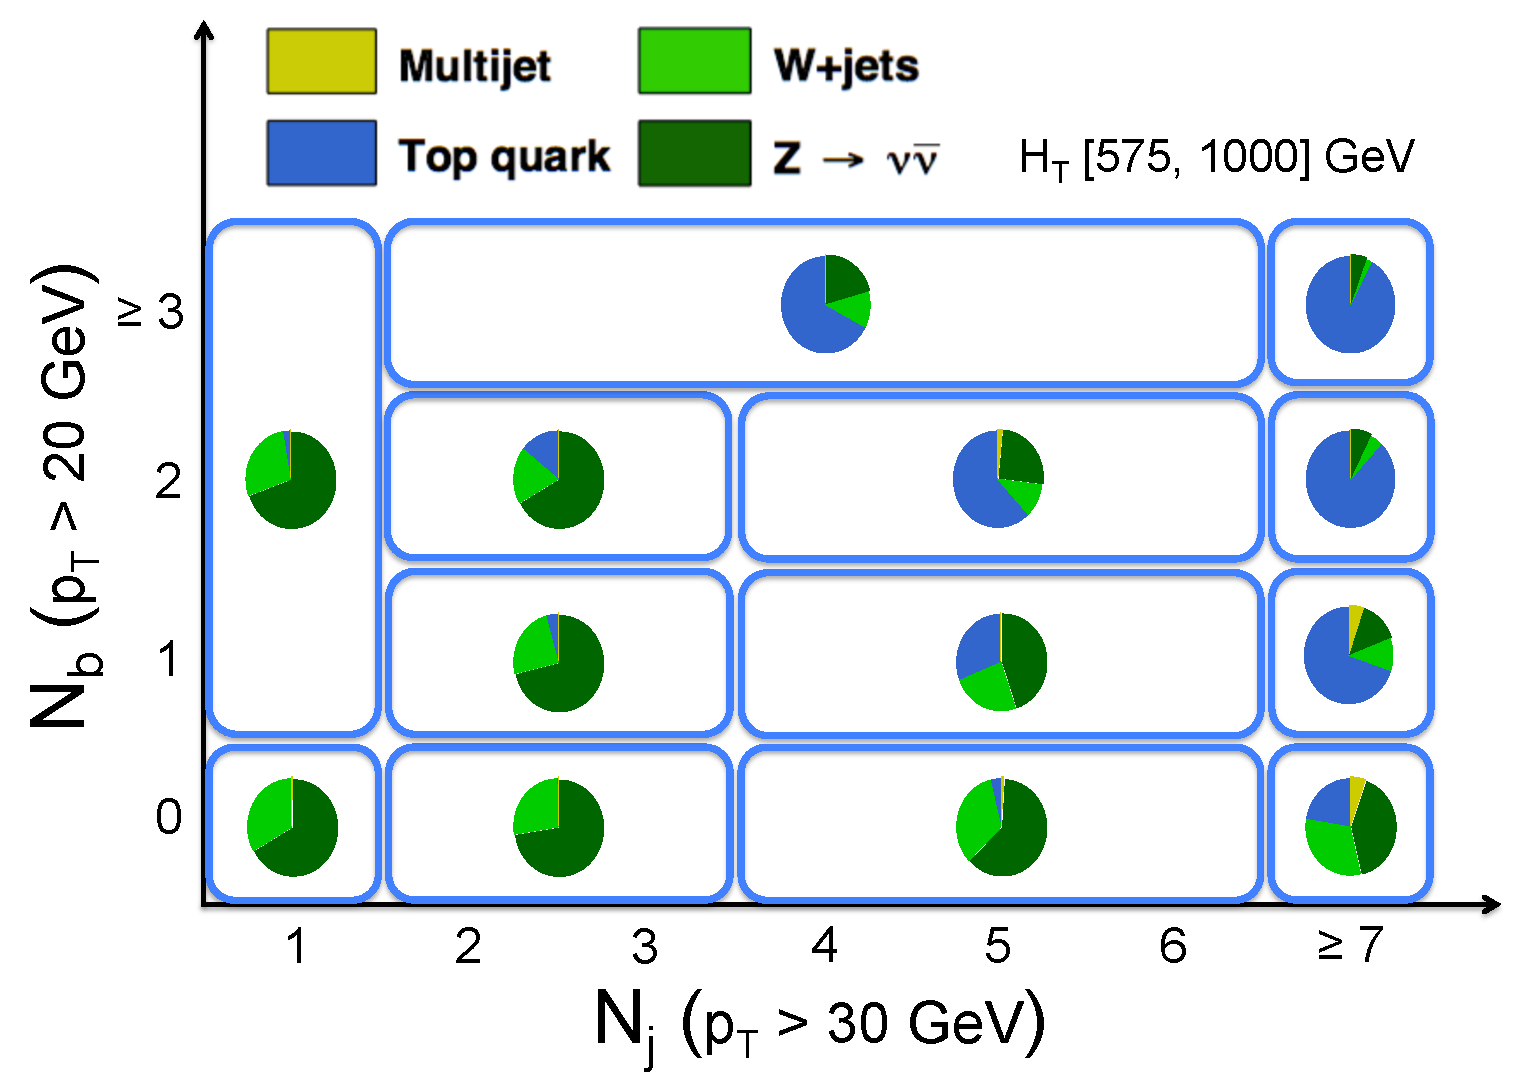
\includegraphics[width=0.75\textwidth]{analysis/figs/bkgComposition_HTlabel}
	\renewcommand{\baselinestretch}{1.0}
	\caption[Topological regions in \nj and \nb for the medium \HT region.]{Topological regions in \nj and \nb for the [575,1000] \HT region. Within each region, the relative fraction of background events from different SM processes is shown based on simulation.}
	\label{fig:topologicalRegions}
\end{figure}
The different topological regions for one \HT region and their background composition are depicted in figure \ref{fig:topologicalRegions}. Each topological region is further divided into \mttwo bins. The \mttwo binning is constructed such that the low edge of the first bin is 400\GeV in regions with \HT > 1500\GeV and 200\GeV everywhere else, and the low edge of the final bin is constructed to contain approximately one background event based on simulation and not exceeding the maximum \HT value in that topological region (since an upper limit on \HT places an upper limit on \mttwo). The detailed \mttwo binning is as follows:
\begin{itemize}
	\item Very Low \HT: [200,300], [300,400], [400,$\infty$]
	\item Low \HT: [200,300], [300,400], [400,500], [500,$\infty$]
	\item Medium \HT: [200,300], [300,400], [400,600], [600,800], [800,$\infty$]
	\item High \HT: [200,400], [400,600], [600,800], [800, 1000], [1000, 1200], [1200,$\infty$]
	\item Extreme \HT: [400,600], [600,800], [800,1000], [1000,1400], [1400,$\infty$]
\end{itemize}
The various \HT bins and associated \mttwo binning can be seen in figure \ref{fig:mt2bins}, and the full breakdown of signal regions (including \mttwo binning) is listed in tables \ref{tbl:mt2bins1} and \ref{tbl:mt2bins2} .
\begin{figure}
	\centering
	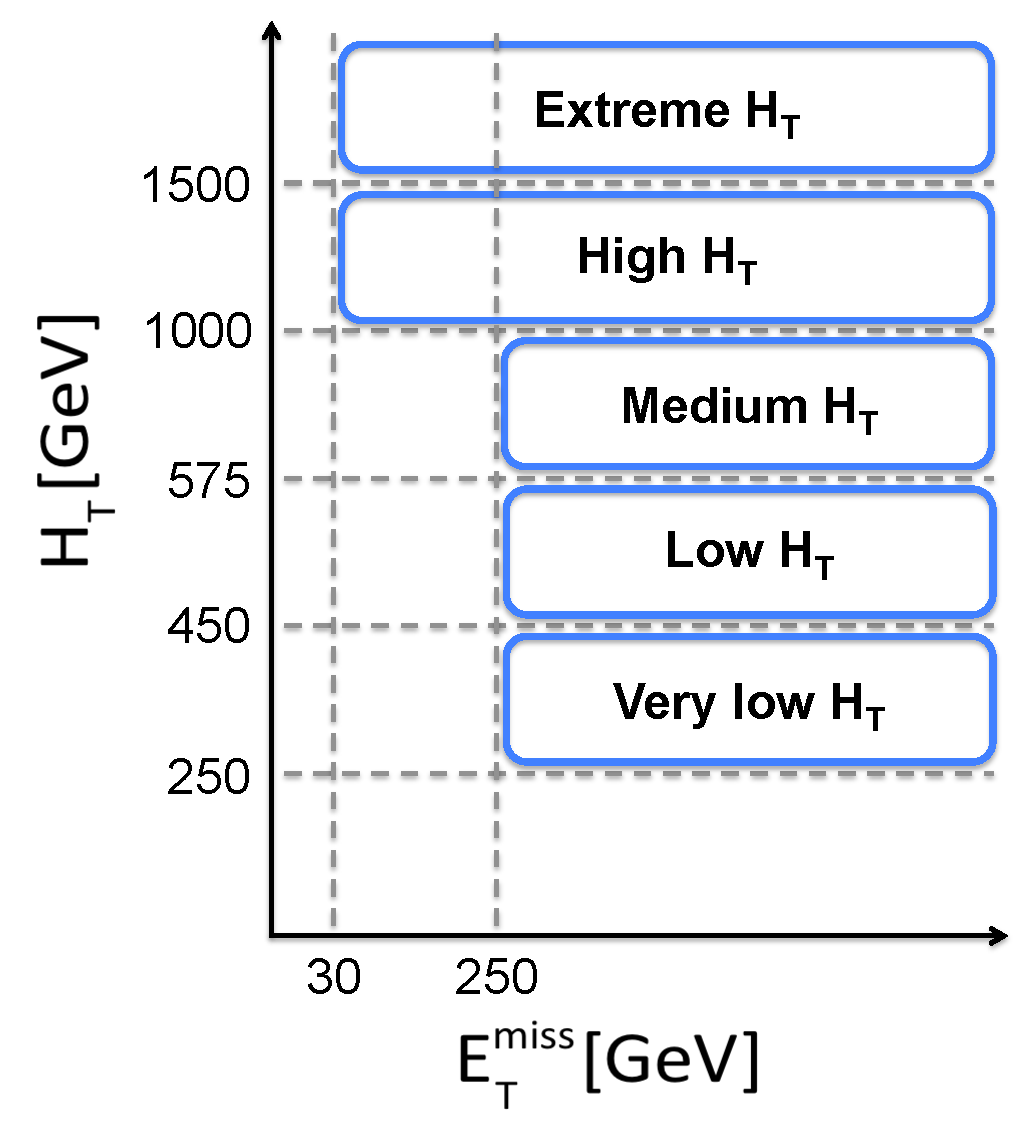
\includegraphics[width=0.38\textwidth]{analysis/figs/HTvsMET_2017}
	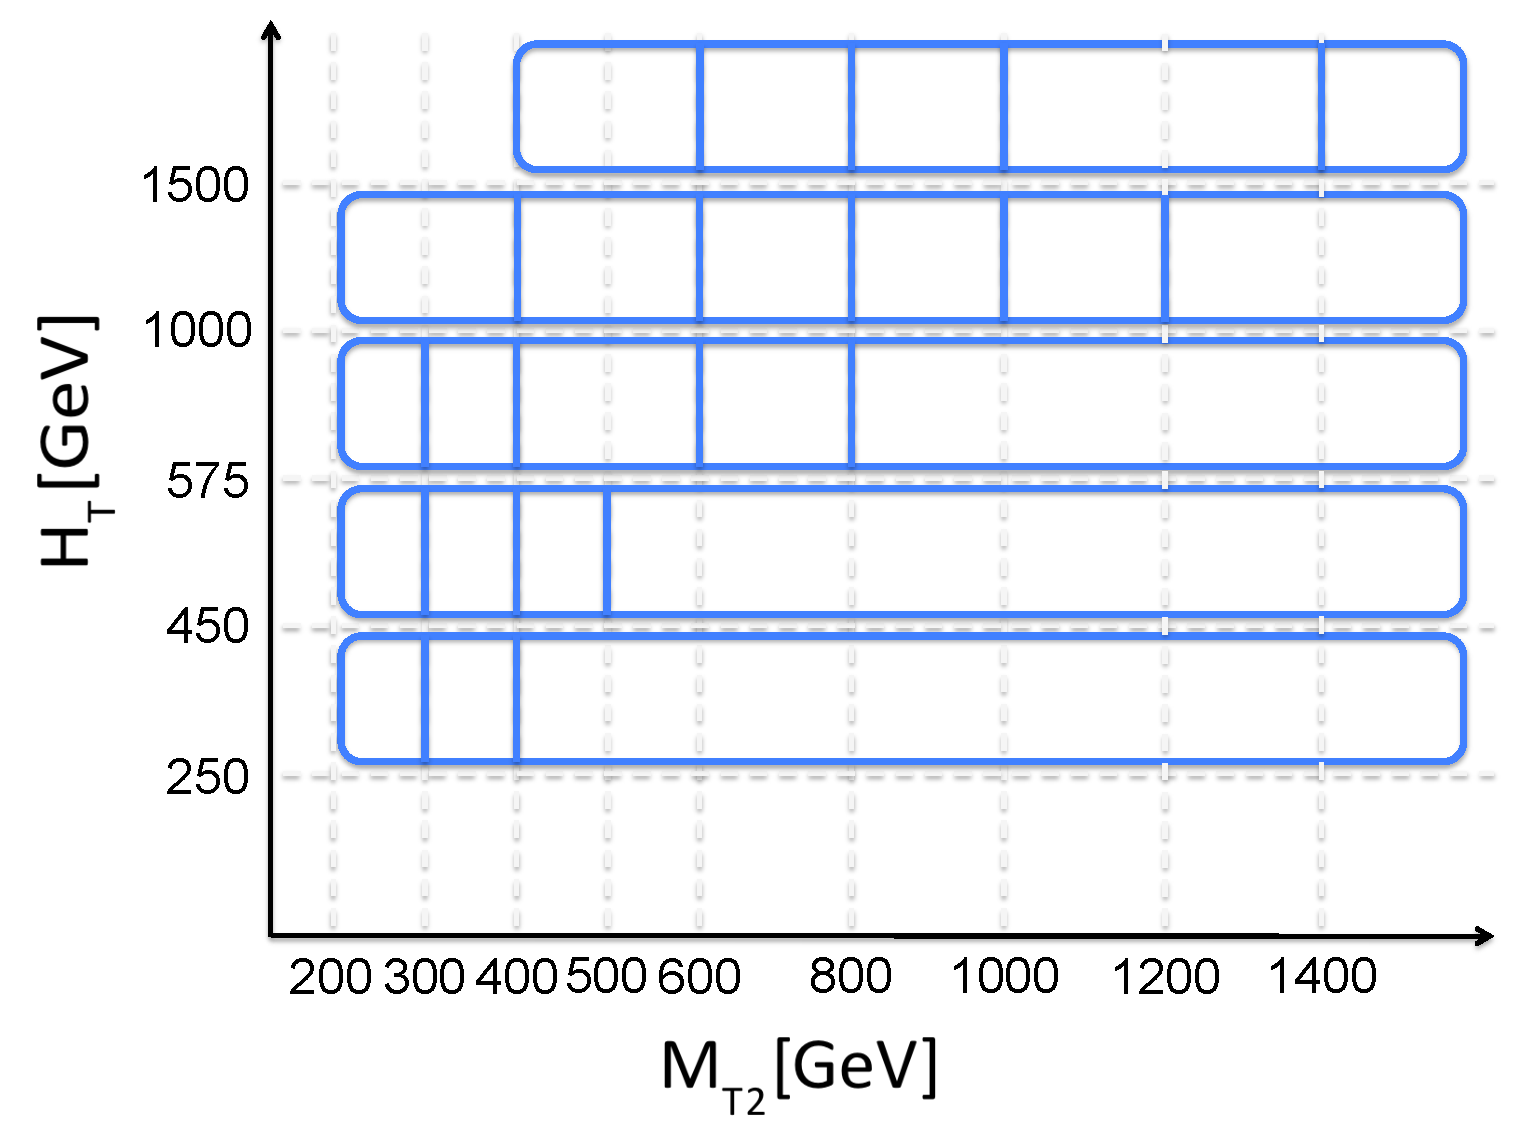
\includegraphics[width=0.55\textwidth]{analysis/figs/HTvsMT2bins_Moriond2017}
	\renewcommand{\baselinestretch}{1.0}
	\caption[Signal region bins in \HT and \MET (left) and \mttwo binning within each \HT region (right).]{Signal region bins in \HT and \MET (left) and \mttwo binning within each \HT region (right). If simulation predicts less than one background event in the greatest \mttwo bin within a region, it is merged with the previous bin.}
	\label{fig:mt2bins}
\end{figure}
\begin{table}[htbp]
	\centering
	\renewcommand{\baselinestretch}{1.0}
	\caption{\mttwo binning in the Very Low, Low, and Medium \HT topological regions.}
	\renewcommand{\arraystretch}{0.65}
	\begin{tabular}{ccl}

\hline

\HT Range [GeV] & Jet Multiplicities & Binning [GeV] \\

\hline%

[ 250, 450 ] & $2-3$j, $  0$b  &  [ 200, 300, 400,  $\infty$ ] \\

 & $2-3$j, $  1$b  &  [ 200, 300, 400,  $\infty$  ] \\

 & $2-3$j, $  2$b  &  [ 200, 300, 400,  $\infty$  ] \\

 & $\geq4$j, $  0$b  &  [ 200, 300, 400,  $\infty$  ] \\

 & $\geq4$j, $  1$b  &  [ 200, 300, 400,  $\infty$  ] \\

 & $\geq4$j, $  2$b  &  [ 200, 300, 400,  $\infty$  ] \\

 & $\geq2$j, $  \geq3$b  &  [ 200, 300, 400,  $\infty$  ] \\ \hline

[ 450, 575 ] & $2-3$j, $  0$b  &  [ 200, 300, 400, 500,  $\infty$  ] \\

 & $2-3$j, $  1$b  &  [ 200, 300, 400, 500,  $\infty$  ] \\

 & $2-3$j, $  2$b  &  [ 200, 300, 400, 500,  $\infty$  ] \\

 & $4-6$j, $  0$b  &  [ 200, 300, 400, 500,  $\infty$  ] \\

 & $4-6$j, $  1$b  &  [ 200, 300, 400, 500,  $\infty$  ] \\

 & $4-6$j, $  2$b  &  [ 200, 300, 400, 500,  $\infty$  ] \\

 & $\geq7$j, $  0$b  &  [ 200, 300, 400,  $\infty$  ] \\

 & $\geq7$j, $  1$b  &  [ 200, 300, 400,  $\infty$  ] \\

 & $\geq7$j, $  2$b  &  [ 200, 300, 400,  $\infty$  ] \\

 & $2-6$j, $  \geq3$b  &  [ 200, 300, 400, 500,  $\infty$  ] \\

 & $\geq7$j, $  \geq3$b  &  [ 200, 300, 400,  $\infty$  ] \\ \hline

[ 575, 1000 ] & $2-3$j, $  0$b  &  [ 200, 300, 400, 600, 800,  $\infty$  ] \\

 & $2-3$j, $  1$b  &  [ 200, 300, 400, 600, 800,  $\infty$  ] \\

 & $2-3$j, $  2$b  &  [ 200, 300, 400, 600, 800,  $\infty$  ] \\

 & $4-6$j, $  0$b  &  [ 200, 300, 400, 600, 800,  $\infty$  ] \\

 & $4-6$j, $  1$b  &  [ 200, 300, 400, 600, 800,  $\infty$  ] \\

 & $4-6$j, $  2$b  &  [ 200, 300, 400, 600, 800,  $\infty$  ] \\

 & $\geq7$j, $  0$b  &  [ 200, 300, 400, 600, 800,  $\infty$  ] \\

 & $\geq7$j, $  1$b  &  [ 200, 300, 400, 600,  $\infty$  ] \\

 & $\geq7$j, $  2$b  &  [ 200, 300, 400, 600,  $\infty$  ] \\

 & $2-6$j, $  \geq3$b  &  [ 200, 300, 400, 600,  $\infty$  ] \\

 & $\geq7$j, $  \geq3$b  &  [ 200, 300, 400, 600,  $\infty$  ] \\ \hline
 
	 \end{tabular}
	\label{tbl:mt2bins1}
\end{table}
\begin{table}
	\centering
	\renewcommand{\baselinestretch}{1.0}
	\caption{\mttwo binning in the High and Extreme \HT topological regions.}
	\renewcommand{\arraystretch}{0.65}
	\begin{tabular}{ccl}

\hline

\HT Range [GeV] & Jet Multiplicities & Binning [GeV] \\

\hline%

[ 1000, 1500 ] & $2-3$j, $  0$b  &  [ 200, 400, 600, 800, 1000, 1200,  $\infty$  ] \\

 & $2-3$j, $  1$b  &  [ 200, 400, 600, 800, 1000, 1200,  $\infty$  ] \\

 & $2-3$j, $  2$b  &  [ 200, 400, 600, 800, 1000,  $\infty$  ] \\

 & $4-6$j, $  0$b  &  [ 200, 400, 600, 800, 1000, 1200,  $\infty$  ] \\

 & $4-6$j, $  1$b  &  [ 200, 400, 600, 800, 1000, 1200,  $\infty$  ] \\

 & $4-6$j, $  2$b  &  [ 200, 400, 600, 800, 1000,  $\infty$  ] \\

 & $\geq7$j, $  0$b  &  [ 200, 400, 600, 800, 1000,  $\infty$  ] \\

 & $\geq7$j, $  1$b  &  [ 200, 400, 600, 800,  $\infty$  ] \\

 & $\geq7$j, $  2$b  &  [ 200, 400, 600, 800,  $\infty$  ] \\

 & $2-6$j, $  \geq3$b  &  [ 200, 400, 600,  $\infty$  ] \\

 & $\geq7$j, $  \geq3$b  &  [ 200, 400, 600,  $\infty$  ] \\ \hline

[ 1500, $\infty$  ] & $2-3$j, $  0$b  &  [ 400, 600, 800, 1000, 1400,  $\infty$  ] \\

 & $2-3$j, $  1$b  &  [ 400, 600, 800, 1000,  $\infty$  ] \\

 & $2-3$j, $  2$b  &  [ 400,  $\infty$  ] \\

 & $4-6$j, $  0$b  &  [ 400, 600, 800, 1000, 1400,  $\infty$  ] \\

 & $4-6$j, $  1$b  &  [ 400, 600, 800, 1000, 1400,  $\infty$  ] \\

 & $4-6$j, $  2$b  &  [ 400, 600, 800,  $\infty$  ] \\

 & $\geq7$j, $  0$b  &  [ 400, 600, 800, 1000,  $\infty$  ] \\

 & $\geq7$j, $  1$b  &  [ 400, 600, 800,  $\infty$  ] \\

 & $\geq7$j, $  2$b  &  [ 400, 600, 800,  $\infty$  ] \\

 & $2-6$j, $  \geq3$b  &  [ 400, 600, $\infty$  ] \\

 & $\geq7$j, $  \geq3$b  &  [ 400, $\infty$ ] \\ 

\hline
	\end{tabular}
	\label{tbl:mt2bins2}
\end{table}
In addition to multijet search regions, this analysis also considers monojet events. Because there is only a single jet (and \mttwo is ill-defined without multiple jets), binning in these regions is defined using \nb and \HT as follows:
\begin{itemize}
	\item \nb: 0b, $\geq$1b
	\item \HT: [250,350], [350,450], [450,575], [575,700], [700,1000], [1000,1200], [1200,$\infty$]
\end{itemize}
As with the multijet regions, monojet \HT bins with less than one simulated background event in the final bin are merged with the penultimate bin.

In addition to these signal regions used to interpret results in the context of various BSM physics models, the analysis also provides results in "super signal regions" (SSRs) as defined in table \ref{tbl:ssr}. These regions provide a simpler set of selections than the nominal signal regions so that phenomenologists may easily reinterpret results in the context of different signal models. Results obtained using the SSRs are not as sensitive as the nominal binning --- finely binned regions have a higher signal-to-background ratio and the global background fit reduces the background uncertainties --- but are much easier to use for reinterpretation than the many correlated bins of the full analysis.
\begin{table}
	\centering
	\renewcommand{\baselinestretch}{1.0}
	\caption{Definition of "super signal regions" used in reinterpretations of the analysis.}
	\begin{tabular}{l||c|c|c|c}
\hline\hline
Region & \nj & \nb & \HT [GeV] & \mttwo [GeV] \\
\hline\hline
2j loose & $\geq 2$ & - & $> 1000$ & $> 1200$ \\
2j tight & $\geq 2$ & - & $> 1500$ & $> 1400$ \\
\hline
4j loose & $\geq 4$ & - & $> 1000$ & $> 1000$ \\
4j tight & $\geq 4$ & - & $> 1500$ & $> 1400$ \\
\hline
7j loose & $\geq 7$ & - & $> 1000$ & $> 600$ \\
7j tight & $\geq 7$ & - & $> 1500$ & $> 800$ \\
\hline
2b loose & $\geq 2$ & $\geq 2$ & $> 1000$ & $> 600$ \\
2b tight & $\geq 2$ & $\geq 2$ & $> 1500$ & $> 600$ \\
\hline
3b loose & $\geq 2$ & $\geq 3$ & $> 1000$ & $> 400$ \\
3b tight & $\geq 2$ & $\geq 3$ & $> 1500$ & $> 400$ \\
\hline
7j3b loose & $\geq 7$ & $\geq 3$ & $> 1000$ & $> 400$ \\
7j3b tight & $\geq 7$ & $\geq 3$ & $> 1500$ & $> 400$ \\
\hline
	\end{tabular}
	\label{tbl:ssr}
\end{table}

\section{Control Regions}
\label{sec:controlRegions}
In order to anchor the data-driven background estimates used in this analysis, {\it control regions} (CR) orthogonal to the signal region selection are defined for various processes. In particular, there are control regions corresponding to enriched samples of single lepton events, \zll events, and QCD multijet events.
%
%\subsection{$\gamma$ + jet Control Region}
%\label{subsec:gammaCR}
%
%\fm{photon plus jets CR selection}

\subsection{Single Lepton Control Region}
\label{subsec:leptonCR}
The single lepton CR is constructed to select a sample enriched with single lepton events, the most dominant contributions being from \ttbar and \Wj production. The same baseline selections described in section \ref{sec:eventSelection} are applied with the exception of the following:
\begin{itemize}
	\item In lieu of the lepton veto, exactly one lepton candidate passing the reco or PF lepton selections is required. In order to avoid double counting (for leptons which are reconstructed both as a reco lepton and PF candidate), PF leptons within \DR < 0.1 of a reco lepton are not considered. 
	\item The transverse mass \Mt between the lepton and \MET must be less than 100\GeV to reduce possible signal contamination.
\end{itemize}
Since non-isolated leptons in the fiducial region of the detector are usually successfully reconstructed, the closest jet within \DR < 0.4 of the lepton is removed and the lepton instead counted as a visible object for the purposes of computing \Ht, \Htmiss, \dphilong, \htovermet, and \mttwo (as well as the hemispheres used to calculate \mttwo). Events are further subdivided into the topological regions described in section \ref{sec:searchRegions} using the modified \HT and \nj and \nb, but not in \mttwo to increase the statistical power of the CR. The signal regions with $\geq7$j,$\geq1$b are all predicted using CRs with identical \Ht bins but $\geq7$j,1-2b to increase the statistical power of those CRs (and to avoid signal contamination in regions with $\geq7$j,$\geq3$b). In addition, for regions with $\HT > 1500\GeV$, the minimum \mttwo threshold is set to 200\GeV to increase available statistics. The monojet CR is binned identically to the signal region.

\subsection{Dilepton Control Region}
\label{subsec:zllCR}

Control regions corresponding to opposite-sign same-flavor leptons (OSSF) from \zll events are used to estimate the \znunu background, with corresponding sets of control regions requiring an opposite-sign opposite-flavor (OSOF) pair to estimate the flavor-symmetric background component in the former dilepton CR. The same baseline selections as described in section \ref{sec:eventSelection} are applied with the exception of the follow:
\begin{itemize}
	\item In lieu of the lepton veto, exactly 2 leptons ($ee$, $e\mu$, or $\mu\mu$) passing loose lepton selections are required.
	\item There is no requirement on \MET. Instead, the dilepton system must have a transverse momentum $p_{\mathrm{T}}(\ell\ell) > 200\GeV$ to mimic the kinematics of the \znunu background and suppress the \ttbar contribution.
	\item Without a missing energy requirement, events are selected in data using leptonic trigger paths. Dimuon events are selected using a combination of dimuon and high-\pt single muon triggers, dielectron events using a combination of dielectron and high-\pt single photon paths (which do not require isolation and recover efficiency for high-\pt electrons or those highly co-linear high-\pt Z bosons), and opposite-flavor events are selected using a combination of $e\mu$ triggers and higher threshold single-lepton paths (to again recover efficiency for some events).
	\item To improve trigger efficiency for these regions, the leading lepton is required to have a minimum momentum $\pt > 100\GeV$ and the sub-leading lepton $\pt > 30\GeV$.
	\item When selecting Z boson candidates for the \znunu estimate, the leptons are also required to be OSSF with an invariant mass $|\mll - m_{\mathrm{Z}}| < 20\GeV$, where $m_{\mathrm{Z}}$ is the nominal Z boson mass.
\end{itemize}
Similar to the single lepton control region, the closest jet within \DR < 0.4 of each lepton is removed and the leptons added to the \MET vector for the purposes of computing \Ht, \Htmiss, \dphilong, \htovermet, and \mttwo (as well as the hemispheres used to calculate \mttwo). Additional information on the \mttwo binning for these regions is detailed in section \ref{sec:zinv}.

\subsection{Multijet Control Region}
\label{subsec:multijetCR}

The multijet control region is designed to select  a sample enriched in QCD events to estimate the multijet background. The same baseline selections described in section \ref{sec:eventSelection} are applied with the exception of the \dphilong requirement, which is inverted to select a sample dominated by QCD events with large fake \MET due to jet energy mismeasurements.

The transfer factor which is used to extrapolate the control region yield to the signal region is measured in a separate QCD-dominated region with $\mttwomath < 200\GeV$, described in detail in section \ref{sec:qcd}. Because of the lower \MET requirement, different trigger paths must be used. For regions with $\HT > 1000\GeV$, trigger paths seeded by a single high-\pt jet are used. For other \HT regions, similar trigger paths with lower jet \pt thresholds are used, but due to the rate of QCD events creating low-\pt jets these paths are prescaled to suppress the data acquisition rate.

This chapter makes use of figures and tables from the \mttwo paper and internal analysis note to illustrate the analysis design, methodology, and results. This work was made possible by contributions from the rest of the Surf \& Turf group, our collaborators at ETH Zurich, and the many other CMS members in the SUSY group and beyond.

% --------------------------------------------------------------------------- %
% --------------------------------------------------------------------------- %
